\section{задание: Генерация текста по заданной структуре}
\subsection{исходные данные}
\indent Тема: \textbf{NoSQL базы данных} \\
\indent Тип документа: \textbf{Статья в блог} \\
\indent Целевая аудитория: \textbf{Студенты IT} \\
\indent Обязательные разделы: \textbf{ \\ \indent \indent Типы БД, CAP-теорема, Примеры использования} \\
\indent Тональность: \textbf{Неформальная}
\subsection{базовый промпт}
\begin{verbatim}
					Ты Сеньёр-разработчик с 10-ти летним опытом работы.
					Напиши {ТИП_ДОКУМЕНТА} на тему {ТЕМА},
					обязательно включая разделы: {РАЗДЕЛЫ}.
					Твоя целевая аудитория: {АУДИТОРИЯ},
					а тональность текста: {ТОНАЛЬНОСТЬ}.
\end{verbatim}
Я выбрал роль Сеньёр-разработчика для ии так как обычно они с таким стажем уже много где работали и точно встречали разные виды баз данных.
\subsection{журнал промпт-инжиниринга}
\noindent Промпт v1:
\begin{verbatim}
					Ты Сеньёр-разработчик с 10-ти летним опытом работы.
					Напиши Статья в блог на тему NoSQL базы данных,
					обязательно включая разделы: Типы БД, CAP-теорема,
							Примеры использования.
					Твоя целевая аудитория: Студенты IT,
					а тональность текста: Неформальная.
\end{verbatim}
\newpage
\noindent Результат (YandexGPT):
\begin{figure}[H]
	\centering
	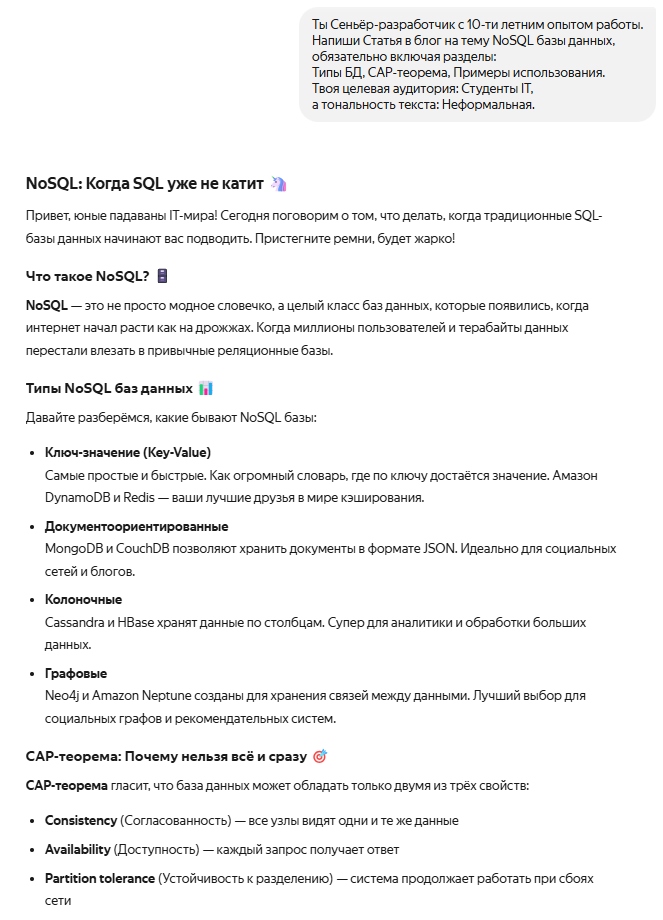
\includegraphics[width=16cm]{z1/a1.png}
\end{figure}
\newpage
\begin{figure}[H]
	\centering
	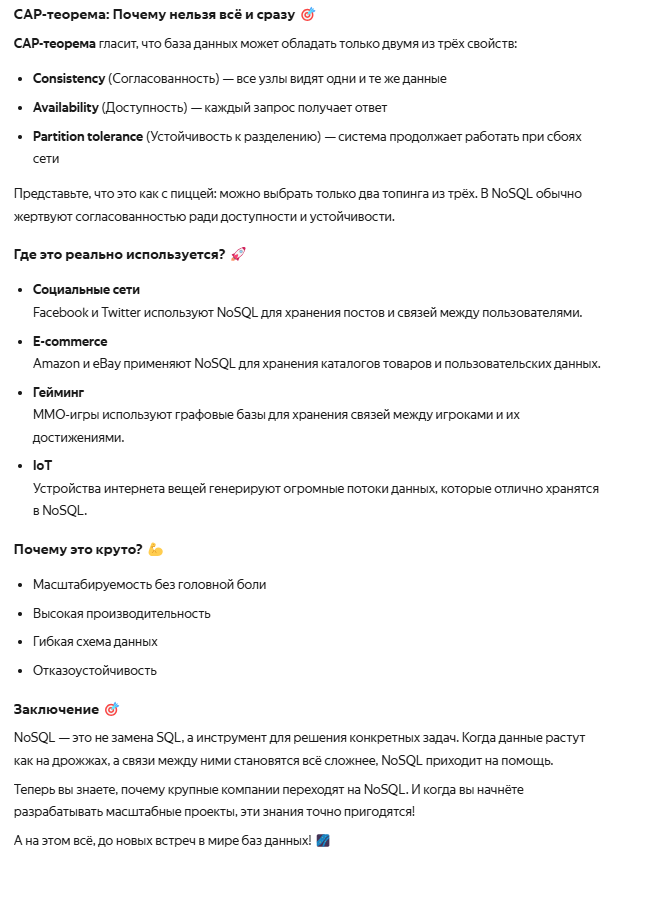
\includegraphics[width=16cm]{z1/a2.png}
	% \caption{Яндекс. Промпт v1: запрос и ответ}
\end{figure}
\newpage
\noindent Анализ ошибок: Ответ слишком длинный \\
Корректировка: попросил писать кратко. \\
\newline
\noindent Промпт v2:
\begin{verbatim}
					Ты Сеньёр-разработчик с 10-ти летним опытом работы.
					Напиши Статья в блог на тему NoSQL базы данных,
					обязательно включая разделы: Типы БД, CAP-теорема,
							Примеры использования.
					Твоя целевая аудитория: Студенты IT,
					а тональность текста: Неформальная.
					Пиши максимально кратко, оставляя только самое важное.
\end{verbatim}
\newpage
Результат (YandexGPT):
\begin{figure}[H]
	\centering
	
\includegraphics[width=14cm]{z1/b1.png}
\end{figure}
% \newpage
\noindent Анализ ошибок: модель предоставила краткий вариант текста. \\
Корректировка: не требуется.
\newpage
\noindent Результат (DeepSeek):
\begin{figure}[H]
	\centering
	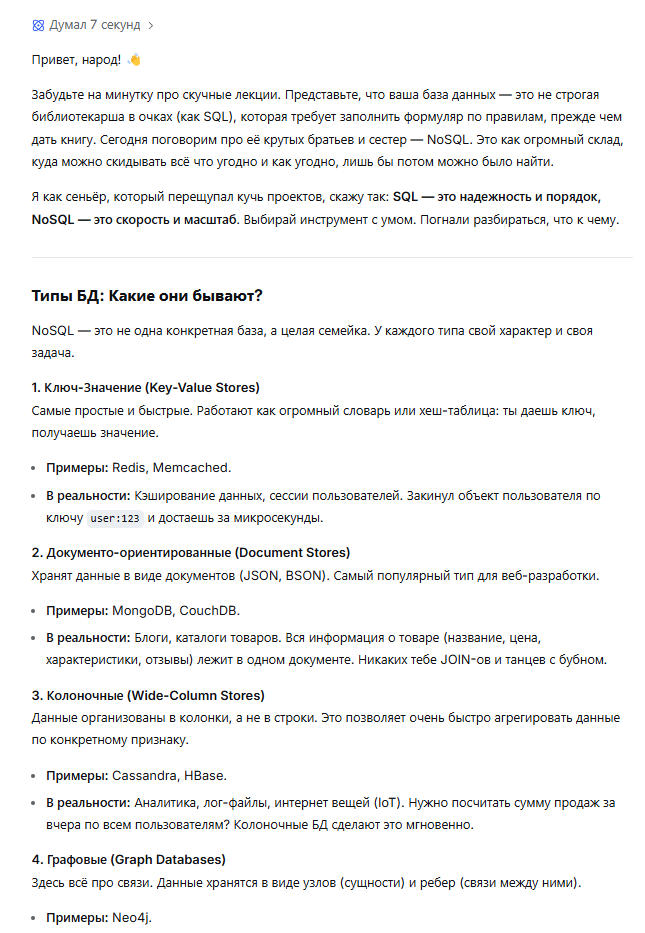
\includegraphics[width=15cm]{z1/c1.png}
\end{figure}
\newpage
\begin{figure}[H]
	\centering
	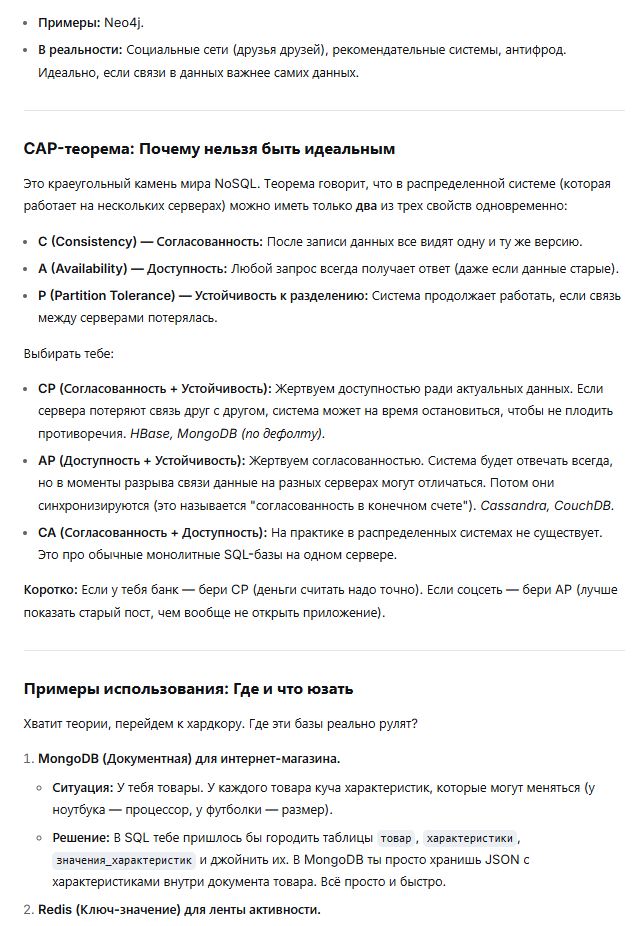
\includegraphics[width=16cm]{z1/c2.png}
\end{figure}
\newpage
\begin{figure}[H]
	\centering
	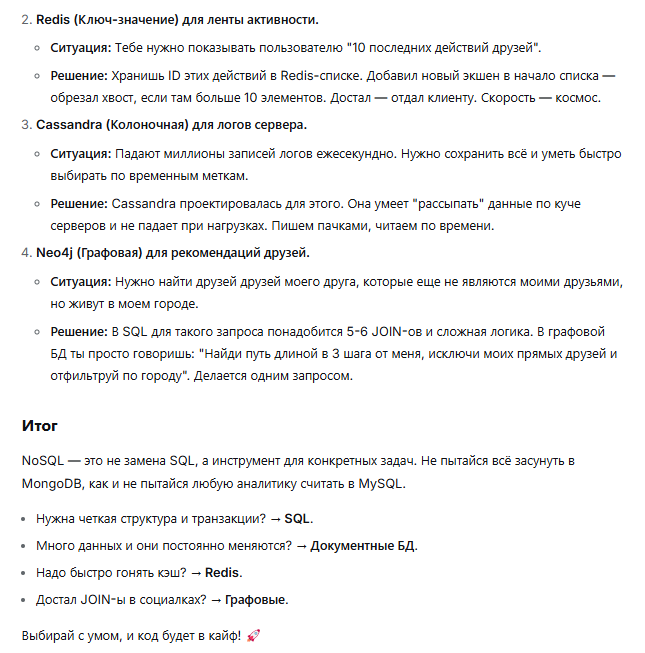
\includegraphics[width=16cm]{z1/c3.png}
\end{figure}
\noindent Анализ ошибок: модель не следует инструкции. \\
Корректировка: не требуется, рекомендуется использовать другую модель. \\
\newpage
\subsection{Сравнение моделей:}
\begin{table}[h!]
	\centering
	\begin{tabular}{|l|p{5cm}|p{5cm}|}
		\hline
		\textbf{Критерий} & \textbf{YandexGPT} & \textbf{DeepSeek} \\
		\hline
		Следование инструкции & 5 & 3 \\
		\hline
		Отсутствие галлюцинаций & 5 & 5 \\
		\hline
		Форматирование & 5 & 5 \\
		\hline
		Длинна текста & 5 & 3 \\
		\hline
		Источники информации & 3 & 5 \\
		\hline
		\textbf{Итог} & 4.6 & 4.2 \\
		\hline
	\end{tabular}
\end{table}
Модель DeepSeek лучше ищет информацию, но плохо сжимает ответ. \\
А модель YandexGPT быстро но плохо ищет информацию, зато хорошо работает с файлами, текстом и фото. \\
\subsection{Финальный промпт:}
\begin{verbatim}
					Ты Сеньёр-разработчик с 10-ти летним опытом работы.
					Напиши {ТИП_ДОКУМЕНТА} на тему {ТЕМА},
					обязательно включая разделы: {РАЗДЕЛЫ}.
					Твоя целевая аудитория: {АУДИТОРИЯ},
					а тональность текста: {ТОНАЛЬНОСТЬ}.
					Пиши максимально кратко, оставляя только самое важное.
\end{verbatim}
\subsection{Вывод по заданию:}
\indent В данном задании лучше всего подходит техника <<Ролевое моделирование>>, так как даёт понять меделе какой специалист для составления документа необходим.
	